%%
%% This is file `mcmthesis-demo.tex',
%% generated with the docstrip utility.
%%
%% The original source files were:
%%
%% mcmthesis.dtx  (with options: `demo')
%% 
%% -----------------------------------
%% 
%% This is a generated file.
%% 
%% Copyright (C)
%%     2010 -- 2015 by Zhaoli Wang
%%     2014 -- 2016 by Liam Huang
%% 
%% This work may be distributed and/or modified under the
%% conditions of the LaTeX Project Public License, either version 1.3
%% of this license or (at your option) any later version.
%% The latest version of this license is in
%%   http://www.latex-project.org/lppl.txt
%% and version 1.3 or later is part of all distributions of LaTeX
%% version 2005/12/01 or later.
%% 
%% This work has the LPPL maintenance status `maintained'.
%% 
%% The Current Maintainer of this work is Liam Huang.
%% 
\documentclass{mcmthesis}
\mcmsetup{CTeX = false,   % ^^e4^^bd^^bf^^e7^^94^^a8 CTeX ^^e5^^a5^^97^^e8^^a3^^85^^e6^^97^^b6^^ef^^bc^^8c^^e8^^ae^^be^^e7^^bd^^ae^^e4^^b8^^ba true
        tcn = 74159, problem = D,
        sheet = true, titleinsheet = true, keywordsinsheet = false,
        titlepage = false, abstract = true}
\usepackage{palatino}
\usepackage{lipsum}
\usepackage{indentfirst}%首行缩进
\setlength{\parskip}{0 em}
\title{The \LaTeX{} Template for MCM Version \MCMversion}
\author{\small \href{http://www.latexstudio.net/}
  {
\includegraphics[width=7cm]{mcmthesis-logo}}}
\date{\today}
\begin{document}
\begin{abstract}

\lipsum[1]
\begin{keywords}
keyword1; keyword2
\end{keywords}
\end{abstract}
\maketitle
\tableofcontents \newpage
\section{Introduction}
\subsection{Background}

With the improvement of people's awareness of protecting environment, the trend of migrating from traditional vehicles to electric
vehicles grows rapidly.In 2016, the sale of electric cars worldwide reach 750 thousand while the registrations break the record in
the past. Only in the fourth season in 2017,the sales of electric cars in US has increased 19\%, sharing 1.2\% of the Light vehicle
market.

In order to accelerate to migration from gasoline cars to electric cars, the construction of charging station is one of the significant
factors we should take account for. How far can an electric car goes is limited by how many charging station on the road. As one of
the major manufacturer of EV(electric car), Tesla constructs quantities of charging station in America. Figure \ref{fig:f1} shows
the distributions of Tesla's supercharger station in U.S.

\begin{figure}[h]
\centering
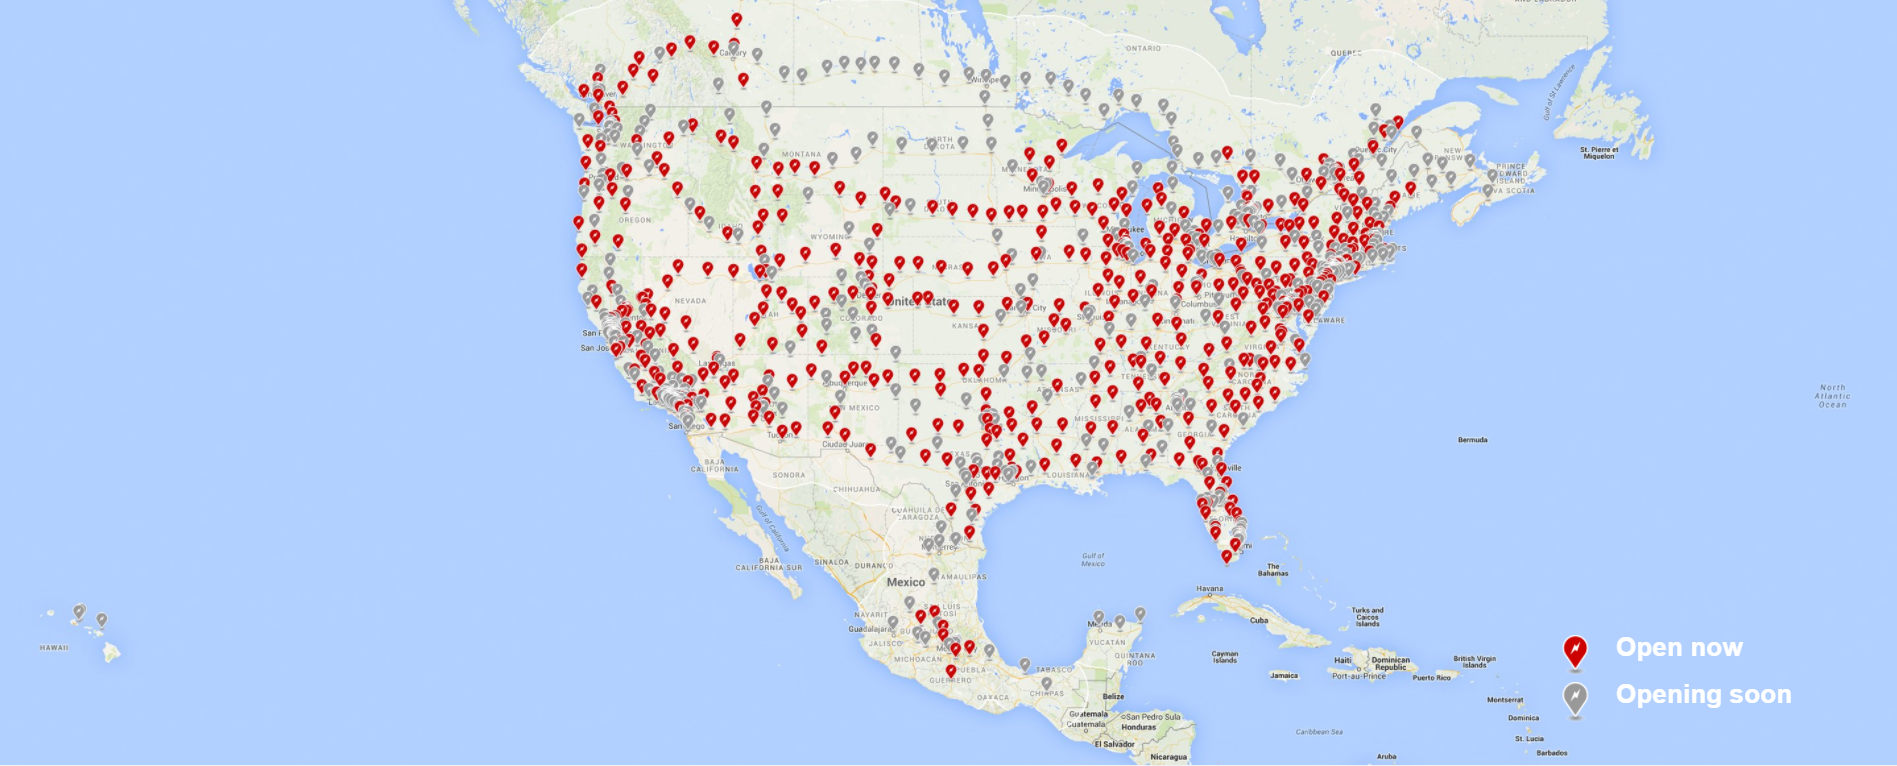
\includegraphics[width=15cm]{1.png}
\caption{Tesla's supercharger stations in U.S.} \label{fig:f1}
\end{figure}

Apart from the number of charging station, the location of these stations is worth considering about. For example, cities will have a
larger demand of charging station than countries. Elements like geographies, population distributions and etc. should be take into account.

\subsection{Problem Restatement and Analysis}
 
In this problem, we are required to accomplish the following five task:
\begin{itemize}
\item find out whether Tesla is able to realize the switch to all-electric in US or not. If succeeds, predict the number and distributions
charging station.
\item discuss optimal number, placement and distributions of charging stations in South Korea, Ireland, or Uruguay and draw a plan to evolving
the charging network.
\item determine whether the schedule above is suitable for some countries with distinguishing geographies, population density distributions,
and wealth distributions. Discuss if it is feasible to establish a classification system which can decide the growth model of switching to
-electric in different countries.
\item comment how will the advanced technologies including car-share and ride-share services, self-driving cars and so forth affect our analysis.
\item write a handout for the leaders of a wide range of countries who will be present at an international energy summit.
\end{itemize}f1
To fulfill the tasks above, we can divide our work into three part roughly. First is the prediction about all-electric and the number of charging
stations, while the number of station depends on the demand for electricity. Secondly, we need to establish a model to determine how to choose the
number and location of stations.Thirdly, we should build a evaluation model to justify whether the charging station model could be applied to
different countries. 

\section{Assumption and Symbol Explanation}

\subsection{Assumption}
\begin{itemize}
  \item   
  \item 
  \item 
  \item 
\end{itemize}

\subsection{Symbol Explanation}
\begin{tabular}{r|l}
  \hline
  symbol & explanation \\
  \hline
\end{tabular}

\section{Task 1}
\subsection{Prediction}

To determine whether Tesla is able to allow the complete switch to all-electric in U.S., we focus on the proportion of the electric
vehicles to all vehicles. Table \ref{aa}

\begin{tabular}{|r|c|c|c|c|c|c|l|}
  year & 2011 & 2012 & 2013 & 2014 & 2015 & 2016 & 2017 \\
\label{tb:t1}
\end{tabular}
\begin{equation}
a^2 \label{aa}
\end{equation}

\[
  \begin{pmatrix}{*{20}c}
  {a_{11} } & {a_{12} } & {a_{13} }  \\
  {a_{21} } & {a_{22} } & {a_{23} }  \\
  {a_{31} } & {a_{32} } & {a_{33} }  \\
  \end{pmatrix}
  = \frac{{Opposite}}{{Hypotenuse}}\cos ^{ - 1} \theta \arcsin \theta
\]
\lipsum[9]

\[
  p_{j}=\begin{cases} 0,&\text{if $j$ is odd}\\
  r!\,(-1)^{j/2},&\text{if $j$ is even}
  \end{cases}
\]

\lipsum[10]

\[
  \arcsin \theta  =
  \mathop{{\int\!\!\!\!\!\int\!\!\!\!\!\int}\mkern-31.2mu
  \bigodot}\limits_\varphi
  {\mathop {\lim }\limits_{x \to \infty } \frac{{n!}}{{r!\left( {n - r}
  \right)!}}} \eqno (1)
\]

\section{Calculating and Simplifying the Model  }
\lipsum[11]

\section{The Model Results}
\lipsum[6]

\section{Validating the Model}
\lipsum[9]

\section{Conclusions}
\lipsum[6]

\section{A Summary}
\lipsum[6]

\section{Evaluate of the Mode}

\section{Strengths and weaknesses}
\lipsum[12]

\subsection{Strengths}
\begin{itemize}
\item \textbf{Applies widely}\\
This  system can be used for many types of airplanes, and it also
solves the interference during  the procedure of the boarding
airplane,as described above we can get to the  optimization
boarding time.We also know that all the service is automate.
\item \textbf{Improve the quality of the airport service}\\
Balancing the cost of the cost and the benefit, it will bring in
more convenient  for airport and passengers.It also saves many
human resources for the airline. \item \textbf{}
\end{itemize}

\begin{thebibliography}{99}
\bibitem{1} D.~E. KNUTH   The \TeX{}book  the American
Mathematical Society and Addison-Wesley
Publishing Company , 1984-1986.
\bibitem{2}Lamport, Leslie,  \LaTeX{}: `` A Document Preparation System '',
Addison-Wesley Publishing Company, 1986.
\bibitem{3}\url{http://www.latexstudio.net/}
\bibitem{4}\url{http://www.chinatex.org/}
\end{thebibliography}

\begin{appendices}

\section{First appendix}

\lipsum[13]

Here are simulation programmes we used in our model as follow.\\

\textbf{\textcolor[rgb]{0.98,0.00,0.00}{Input matlab source:}}
\lstinputlisting[language=Matlab]{./code/mcmthesis-matlab1.m}

\section{Second appendix}

some more text \textcolor[rgb]{0.98,0.00,0.00}{\textbf{Input C++ source:}}
\lstinputlisting[language=C++]{./code/mcmthesis-sudoku.cpp}

\end{appendices}
\end{document}

%% 
%% This work consists of these files mcmthesis.dtx,
%%                                   figures/ and
%%                                   code/,
%% and the derived files             mcmthesis.cls,
%%                                   mcmthesis-demo.tex,
%%                                   README,
%%                                   LICENSE,
%%                                   mcmthesis.pdf and
%%                                   mcmthesis-demo.pdf.
%%
%% End of file `mcmthesis-demo.tex'.
